\chapter{\ifproject%
    \ifenglish Project Structure and Methodology\else โครงสร้างและขั้นตอนการทำงาน\fi
  \else%
    \ifenglish Project Structure\else โครงสร้างของโครงงาน\fi
  \fi
 }

ในบทนี้จะกล่าวถึงภาพรวมของ Chatbot ที่จะสร้างว่ามีการใช้งานอย่างไรการทำงานของ Dialogflow ทำงานอย่างไร
พร้อมทั้งอธิบายการจัดการ database ทั้ง Cloud Storage และ Firestore ว่าวางแผนไว้อย่างไร

\makeatletter

% \renewcommand\section{\@startsection {section}{1}{\z@}%
%                                    {13.5ex \@plus -1ex \@minus -.2ex}%
%                                    {2.3ex \@plus.2ex}%
%                                    {\normalfont\large\bfseries}}

\makeatother
%\vspace{2ex}
% \titleformat{\section}{\normalfont\bfseries}{\thesection}{1em}{}
% \titlespacing*{\section}{0pt}{10ex}{0pt}

\section{โครงสร้าง}
\begin{figure}[hbt!]
  \begin{center}
    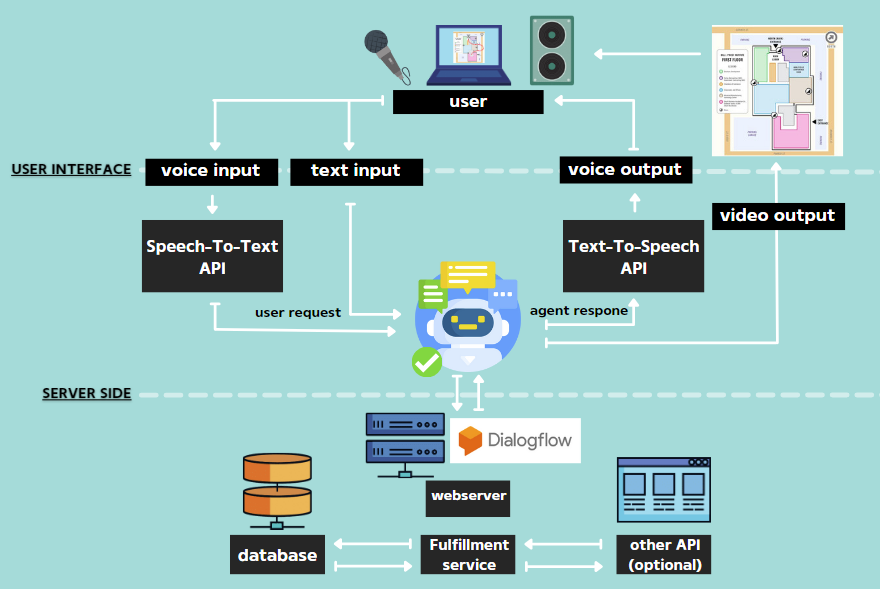
\includegraphics[width=\textwidth,keepaspectratio]{pic/overview.png}
  \end{center}
  \caption{ภาพรวมการทำงานของ Chatbot}
  \label{fig:overview}
\end{figure}
โปรเจคนี้ทำการพัฒนาแชทบอทผ่าน Dialogflow ที่เชื่อมต่อกับ Web application ในฝั่ง client ซึ่งสร้างโดยใช้ Next.Js และทำการเชื่อมต่อกับ
server ที่เขียนด้วย Express ที่ทำงานอยู่บน NodeJS เพื่อเป็นตัวยิง requrest ดึงข้อมูลจาก Database โดยชนิดของ Database ที่ใช้เป็นแบบ NoSQL ซึ่งเมื่อผู้ใช้
ถามคำถามผ่านทางการพูดใส่ไมค์ที่อยู่บริเวณอาคาร ตัว Web จะส่ง user request Google STT ก่อนเพื่อแปลง
เสียงที่ได้รับมาให้กลายเป็นข้อความและตอบกลับมาที่เว็บหลังจากได้ตัวข้อความแล้วก็จะส่ง user request ไปยัง
Dialogflow ซึ่งคำถามที่ส่งมานั้นจะถูกแยกออกเป็น 3 กรณีนั่นคือ

\begin{enumerate}
  \item ไม่ต้องการข้อมูลจาก database หรือ API: คำตอบจะถูกส่งคืนกลับไปเป็น agent response
        ของ Dialogflow
  \item ต้องการข้อมูลจาก database: Dialogflow จะทำการส่ง API ไปที่ Fulfillment จากนั้นจะทำการ
        ดึงข้อมูลจาก database แล้วส่งกลับไปยัง Dialogflow ในรูปแบบของ JSON เพื่อให้ Dialogflow ส่ง
        คำตอบให้ผู้ใช้งานต่อไป
  \item ต้องการข้อมูลจาก API: Dialogflow จะทำการส่ง API ไปที่ Fulfillment จากนั้นจะทำการข้อมูล
        ซึ่ง API จะตอบกลับมาในรูปของ JSON ให้กับ Dialogflow และให้ Dialogflow ส่งคำตอบให้ผู้ใช้งานอีกที่
\end{enumerate}
\section{Database}
\subsection{รูปแบบการเก็บข้อมูลใน Realtime Database}
รูปแบบในการเก็บข้อมูลที่เลือกใช้จะเป็นแบบ NoSQL บน Realtime Database ของ Firebase ซึ่งเราได้วางโครงสร้างไว้ดังนี้
\begin{figure}[hbt!]
  \begin{center}
    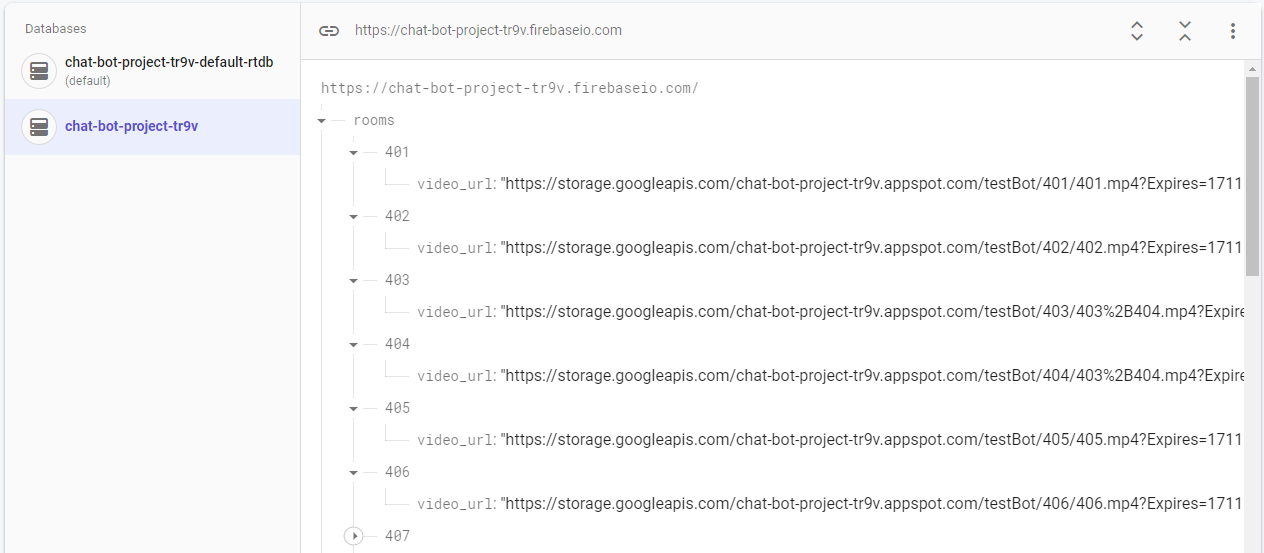
\includegraphics[width=\textwidth,keepaspectratio]{pic/database_mapPath.png}
  \end{center}
  \caption{การเก็บข้อมูลที่อยู่ของไฟล์ video แผนที่สำหรับแต่ละห้อง}
  \label{fig:db_mapPath}
\end{figure}

\begin{figure}[hbt!]
  \begin{center}
    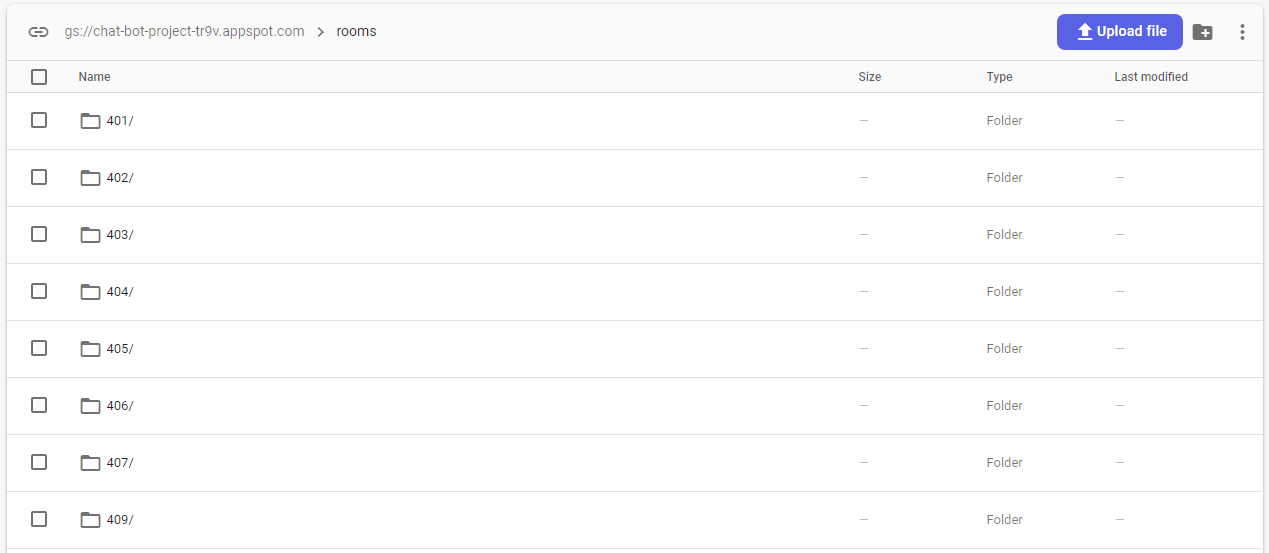
\includegraphics[width=\textwidth,keepaspectratio]{pic/db_storage_folder.png}
  \end{center}
  \caption{folder สำหรับเก็บ video ของแผนที่สำหรับแต่ละห้อง}
  \label{fig:db_storage_floorFolder}
\end{figure}

\begin{figure}[hbt!]
  \begin{center}
    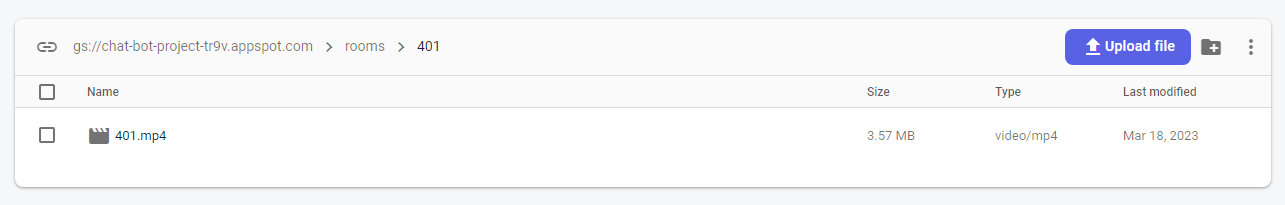
\includegraphics[width=\textwidth,keepaspectratio]{pic/db_storage_file.png}
  \end{center}
  \caption{การเก็บข้อมูลไฟล์ video แผนที่สำหรับแต่ละห้อง}
  \label{fig:db_storage}
\end{figure}

\subsection{รูปแบบการเก็บข้อมูลใน Cloud Storage}
รูปแบบในการเก็บข้อมูลที่อยู่บน Cloud Storage จะมีลักษณะเหมือนกับ Google Drive เราสามารถอัพโหลดไฟล์ขึ้นไปฝากไว้บน Cloud
ได้โดยบนนี้เราจะเก็บไฟล์ video ที่แสดงเส้นทางไปยังห้องต่างๆในแต่ละชั้นดังนี้



\section{การทำงานของ Dialogflow}

Dialogflow ใช้เทคนิค Natural language ในการสื่อสารระหว่างคอมพิวเตอร์เเละภาษามนุษย์ จากจุดเด่นดั้งกล่าว เราจีงเลือก
Dialogflow มาเป็นตัวกลางระหว่างมนุษย์แลคอมพิวเตอร์ Chatbot~\cite{df-overview}
\subsection{การเปลี่ยน Input ให้เป็น Intent}
สามารถแบ่งออกได้เป็น 3 ขั้นตอน
\begin{enumerate}
  \item ผู้ใช้งานพิมพ์ข้อความ (Input) เข้ามา ซึ่งอาจจะเป็นชุดคำพูดหรือประโยค (Utterance)
  \item ระบบจะทำการหาใจความสำคัญที่ผู้ใช้ต้องการที่จะสื่อ (Intent) ให้กับ Chatbot มา process
  \item หลังจากระบุ Intent ได้แล้ว ระบบจะทำขั้นตอน Intent Matching เพื่อหา Response หรือการตอบกลับต่อข้อความนั้น
\end{enumerate}

\begin{figure}[hbt!]
  \begin{center}
    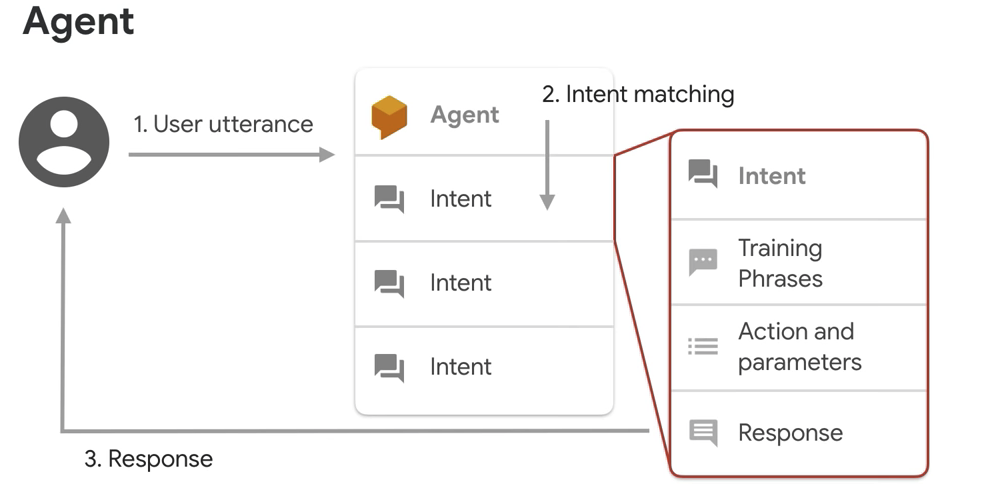
\includegraphics[width=\textwidth,keepaspectratio]{pic/df_input_intent_conventer.png}
  \end{center}
  \caption{การแปลง Input ให้เป็น Intent}
  \label{fig:df-TTI}
\end{figure}
ตัวอย่าง Utterance หรือ ชุดคำพูดหรือประโยคที่เราคาดว่าผู้ใช้งานจะต้องใช้ (Input)
\begin{center}
``Hey Bot, Can you make an appointment for me at 9 p.m.?''
\end{center}
ตัวอย่างการระบุ Intent จะเห็นได้ว่าสิ่งที่ผู้ใช้งานต้องการคือ ทำการนัดหมายที่เวลา 9 p.m. ดังนั้น
Intent ของประโยคนี้คือ `make an appointment for me at 9 p.m.' จากนั้น Bot
จะทำการตอบ  Reponse ที่เราได้เตรียมไว้สำหรับ Intent นี้เป็นลำดับถัดไป
\subsection{ตรวจสอบ intent และตอบกลับ}

\begin{figure}[hbt!]
  \begin{center}
    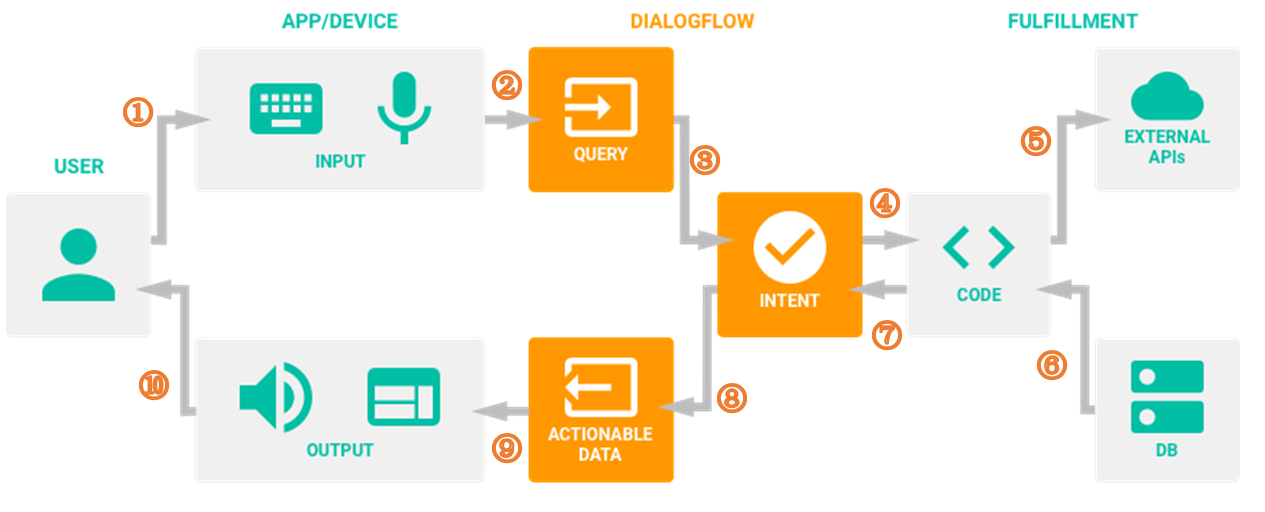
\includegraphics[width=\textwidth,keepaspectratio]{pic/df-overview.jpg}
  \end{center}
  \caption{ภาพรวมการทำงานของ Dialogflow}
  \label{fig:df-overview}
\end{figure}
หลังจากที่ได้ intent มาแล้ว Dialogflow ก็จะทำการเทียบ intent เข้ากับ intent ทั้งหมดที่มีเพื่อหาคำตอบที่ตรงกันที่สุด
เพื่อจะหาว่าผู้ใช้ถามเข้ามาว่าอะไรและควรจะตอบอย่างไรกลับไป
ถ้ามีข้อมูลเพียงพอก็จะตอบกลับไปเลย แต่ถ้าต้องการข้อมูลเพิ่มเติมเช่น ข้อมูลจาก database หรือจาก API อื่นๆก็จะต้องขอ
user request ไปยัง daatabase หรือ API เป้าหมายเพื่อทำ Fulfillment หรือก็คือการเติมเต็มคำตอบและคอยตอบกลับไป
เป็น agent response ให้ กับ user อีกที



\section {Algorithm}
\subsection{Natural Language Processing}
Natural Language Processing หรือ NLP คือ กระบวนการที่ทำให้คอมพิวเตอร์สามารเข้าใจภาษามนุษย์ได้
กระบวนการนี้จะช่วยทำให้คอมพิวเตอร์มีความเข้าใจเกี่ยวกับภาษาที่เราพิมพ์ และยังสามารถตีความจากข้อความได้
ซึ่ง NLP มี subset อยู่ภายในคือ Natural Language Understanding (NLU) โดยจะเน้นการทำงานไปที่ให้คอมพิวเตอร์
ให้สามารถเข้าใจข้อความจากมนุษย์ได้ลึกซึ้งขึ้น โดยฟังก์ชันหลักของ NLU จะมุ่งเน้นหาความสัมพันธ์เชิงความหมายของคำในประโยค,
ดึงใจความสำคัญจากประโยค, เน้นการถามตอบข้อมูลเพิ่มเติม, และเน้นการตอบโต้พูดคุย โดย NLU ถือเป็นหนึ่งในหลักการสำคัญสำหรับ
การทำงานของ Chatbot

\begin{figure}[hbt!]
  \begin{center}
    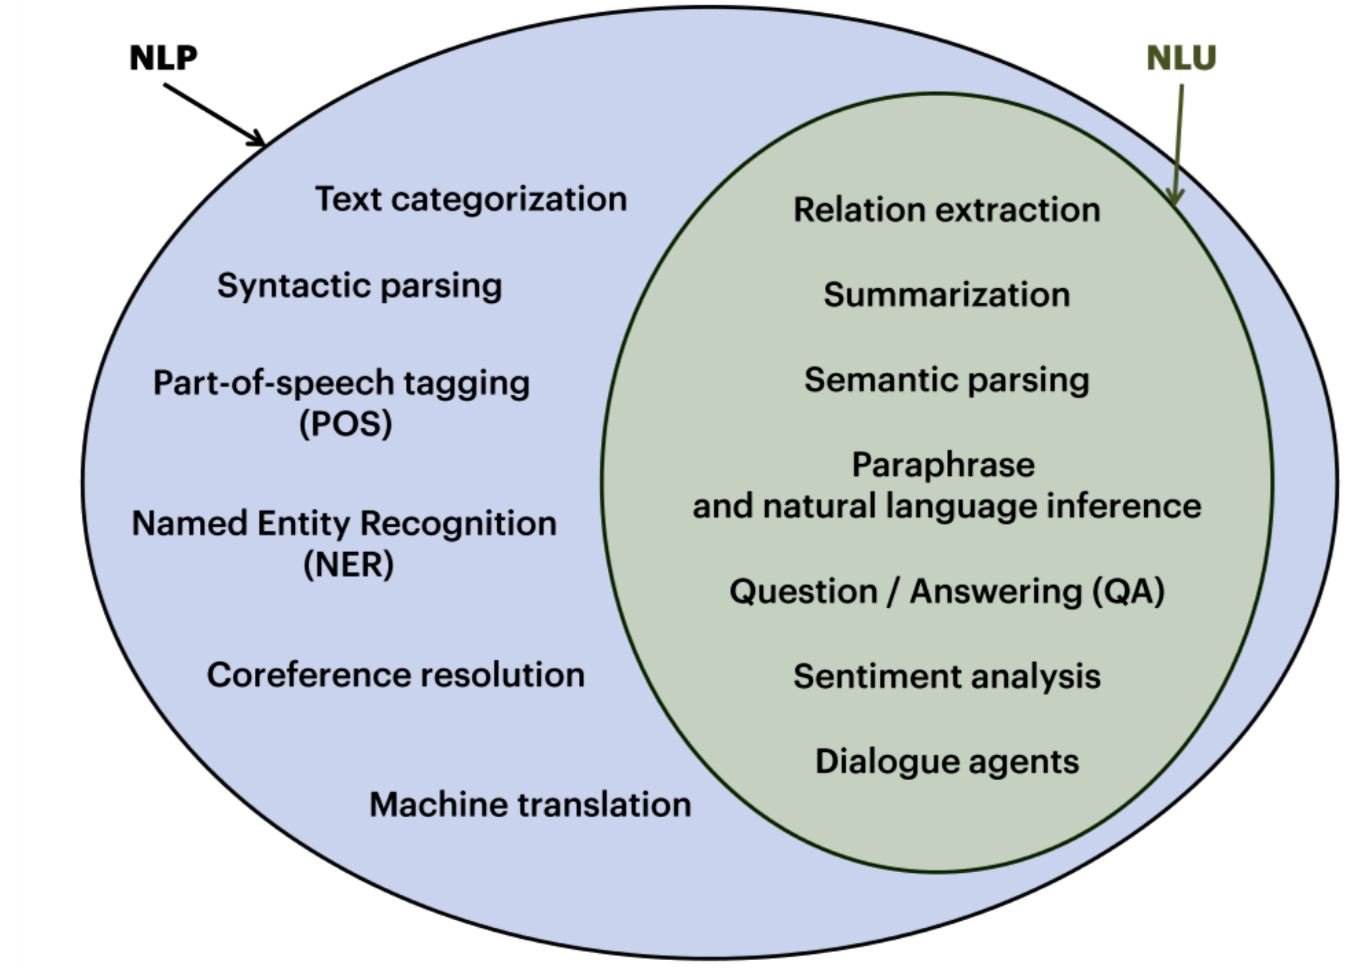
\includegraphics[width=\textwidth,keepaspectratio]{pic/NLPandNUL.png}
  \end{center}
  \caption{Natural Language Processing (NLP) และ Natural Language Understanding (NUL)}
  \label{fig:NLPandNUL}
\end{figure}

